%# -*- coding: utf-8 -*-
\documentclass{ctexart}
%
%页眉页脚
\usepackage{geometry}
\geometry{left=2.5cm,right=2.5cm,top=2.5cm,bottom=2.5cm}
\usepackage{xcolor}
\usepackage{graphicx}
\usepackage{amsmath}
\usepackage{url}
\usepackage{enumerate}
\usepackage{subfigure}
\usepackage{listings} 
\usepackage[colorlinks,linkcolor=black]{hyperref}% 书签
\usepackage{fancyhdr}

\fancyhead[R]{\thepage}% 这是奇数页右页眉、偶数页左页眉
\fancyhead[L]{}
\chead{MATLAB 综合实验之图像处理}%这是中间页眉
\pagestyle{fancy}
\lstset{numbers=left, %设置行号位置
    numberstyle=\tiny, %设置行号大小
    keywordstyle=\color{blue}, %设置关键字颜色
    commentstyle=\color[cmyk]{1,0,1,0}, %设置注释颜色
    frame=single, %设置边框格式
    breaklines, %自动折行
    extendedchars=false, %解决代码跨页时,章节标题,页眉等汉字不显示的问题
    xleftmargin=1.5em,xrightmargin=1.5em, aboveskip=1em, %设置边距
    tabsize=4, %设置tab空格数
    showspaces=false %不显示空格
}
%中文
\usepackage{xeCJK}
%字体设置
\usepackage{indentfirst}
\setlength{\parindent}{2em} %首行缩进
\renewcommand\thesubsection{(\arabic{subsection})}
\renewcommand\thesubsubsection{(\alph{subsubsection})}

\title{MATLAB 综合实验之图像处理\footnote{所有的.m文件均采用utf8编码,windows版matlab中打开可能会出现中文乱码的情况,请用其它编辑器打开}}
\author{聂浩~~ 无31~~ 2013011280}
\date{\today}
\begin{document}
\maketitle
\section{基础知识}
\subsection{
MATLAB 提供了图像处理工具箱,在命令窗口输入 help images 可查看该工具箱内的所有函数。 请阅读并大致了解这些函数的基本功能。}

感觉较为常用的函数有:
\begin{itemize}
    \item{image 建立图片对象,在坐标轴中绘制,颜色取决于现在的颜色设置}
    \item{imshow 显示图片(按照原来图片的大小)}
    \item{imread 读取图片文件}
    \item{imwrite 写图片文件}
    \item{imabsdiff 比较两张图片的差异}
    \item{checkerboard 生成棋盘}
\end{itemize}

\subsection{
利用 MATLAB 提供的 Image file I/O 函数分别完成以下处理:}
\subsubsection{以测试图像的中心为圆心,图像的长和宽中较小值的一半为半径画一个红颜色的圆:}
因为这个图像非常小,所以直接用循环就进行了处理,没有进行太多优化.图像如图\ref{1circle},代码见下一问。
\begin{figure}
    \centering
    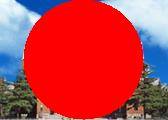
\includegraphics[width=0.3\textwidth]{pic/circle.jpg}\\
    \caption{绘制红色圆\label{1circle}}
\end{figure}

\subsubsection{将测试图像涂成国际象棋状的“黑白格”的样子,其中“黑”即黑色,“白”则意味着保留原图。 用一种看图软件浏览上述两个图,看是否达到了目标。}
图像如图\ref{1board}
\begin{figure}
    \centering
    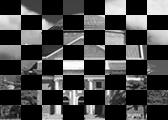
\includegraphics[width=0.3\textwidth]{pic/board.jpg}\\
    \caption{绘制黑白格\label{1board}}
\end{figure}

代码如下(a3\_1.m):
\lstinputlisting[language=matlab]{a3_1.m}

\section{图像压缩编码}
\subsection{
图像的预处理是将每个像素灰度值减去128,
这个步骤是否可以在变换域进行?
请在测试图像中截取一块验证你的结论。}
根据二维DCT变换的定义式$C=DPD^T$,这是一个线性变换,所以变换前后处理是一致的。

在这里截取了hall\_gray(61:68,81:88),两种处理次序后的绝对值差在$10^{-12}$数量级,可以认为这只是计算误差,故两者等价。

代码如下(a3\_2\_1.m):
\lstinputlisting[language=matlab]{a3_2_1.m}

\subsection{
请编程实现二维 DCT ,并和 MATLAB 自带的库函数 dct2 比较是否一致。}
我直接使用计算D矩阵然后相乘的方法进行计算,其计算复杂度为$O(n^2)$。

系统的DCT2函数的调用了两次DCT函数,而DCT函数则使用了FFT,因此其计算复杂度为$O(n\log (n))$。

两者的误差在$10^{-9}$数量级,可以认为这只是计算误差。

在数据较大时,如图\ref{a322},系统DCT2函数快于我的my\_DCT2函数。\footnote{因为计算机差异,具体值可能不同}
\begin{figure}
    \centering
    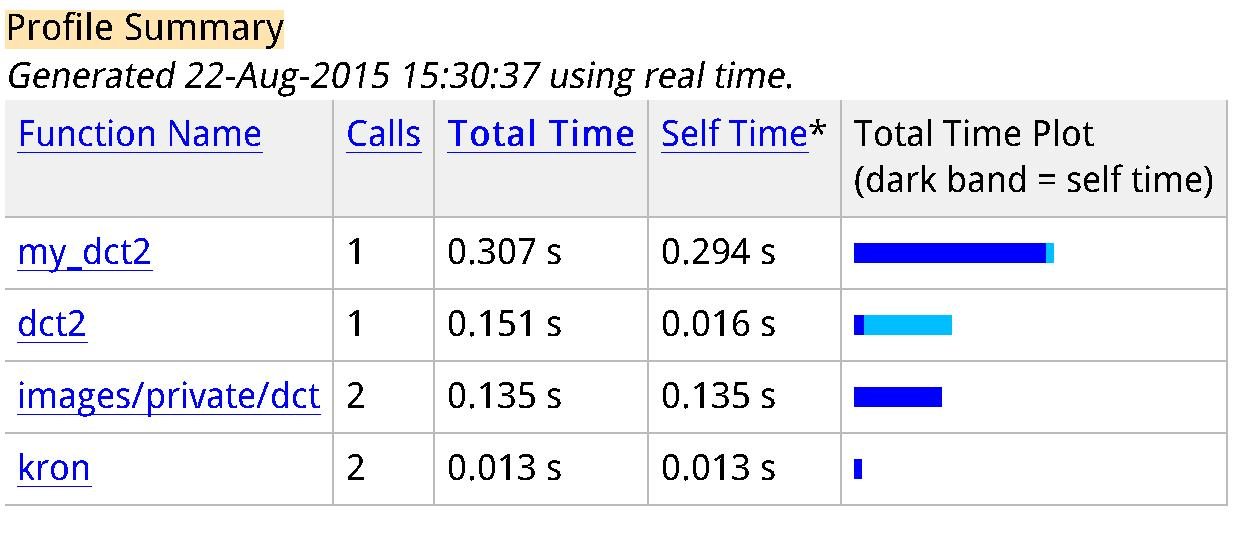
\includegraphics[width=0.8\textwidth]{pic/a3_2_2.jpg}\\
    \caption{将hall\_gray重复100次后两种
    DCT变换所消耗的时间\label{a322}}
\end{figure}

my\_dct2的代码如下:
\lstinputlisting[language=matlab]{my_dct2.m}

测试代码如下(a3\_2\_2.m):
\lstinputlisting[language=matlab]{a3_2_2.m}

\subsection{
如果将 DCT 系数矩阵中右侧四列的系数全部置零,逆变换后的图像会发生什么变化?选取一块图验证你的结论。 如果左侧的四列置零呢?
}
如图\ref{a323},右侧四列都置零,逆变换后的图像变化不大,因为人眼对高频分量不敏感。当左侧四列都置零,逆变换图片变暗。因为很多低频分量,包括基频被滤掉,导致各点值偏小而发暗。
\begin{figure}
    \centering
    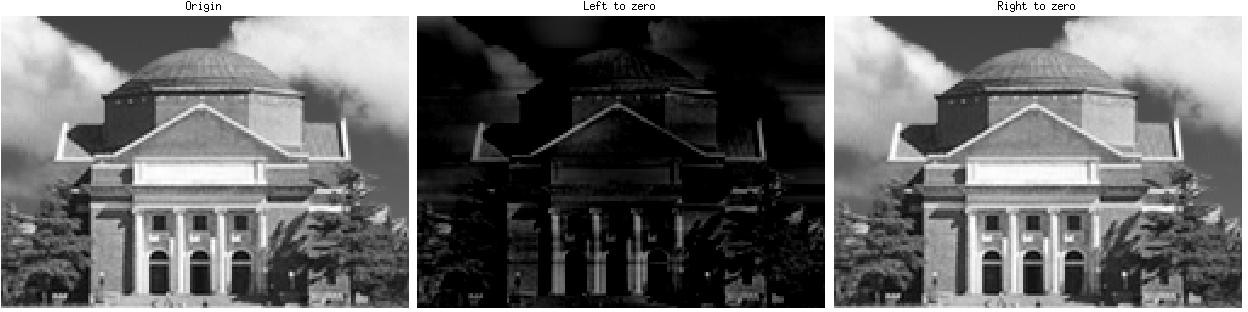
\includegraphics[width=0.8\textwidth]{pic/a3_2_3.jpg}\\
    \caption{原图、左四列与右四列分别清零\label{a323}}
\end{figure}

代码如下(a3\_2\_3.m)
\lstinputlisting[language=matlab]{a3_2_3.m}
\subsection{
若对 DCT 系数分别做转置、 旋转 90 度和旋转 180 度操作 (rot90) ,逆变换后恢复的图像有何变化?选取一块图验证你的结论。}
如图\ref{a324},转置使得图像沿左上至右下的对角线翻转镜像;旋转$90^{\circ}$使图像在之前的基础上还出现了黑白条纹;旋转$180^{\circ}$后图像没有旋转,但是出现了黑白小斑点。

这是因为转置并未改变高低频信息,但两轴被交换,故出现翻转;旋转使得高频和低频分量的信息混淆,故高频相对之前被放大了——旋转$90^{\circ}$只有一个方向的高频较明显,故为条纹;旋转$180^{\circ}$则增强了两个方向的高频分量,故为斑点。
\begin{figure}
    \centering
    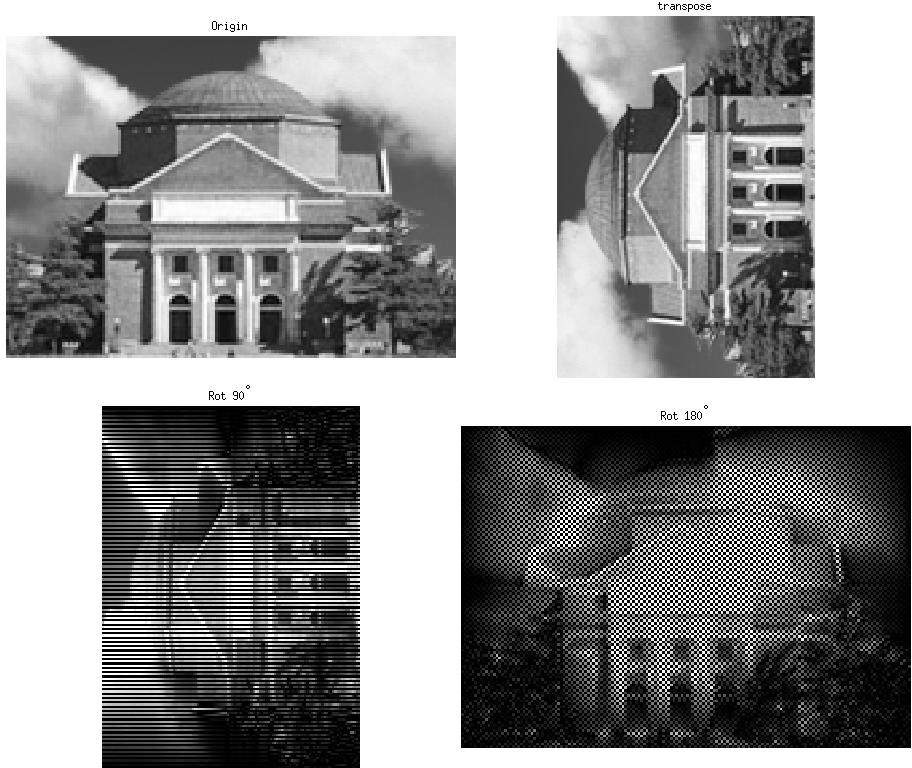
\includegraphics[width=0.8\textwidth]{pic/a3_2_4.jpg}\\
    \caption{左四列与右四列分别清零\label{a324}}
\end{figure}

代码如下(a3\_2\_4.m):
\lstinputlisting[language=matlab]{a3_2_4.m}
\subsection{
如果认为差分编码是一个系统,请绘出这个系统的频率响应,说明它是一个\_\_\_\_(低通、 高通、 带通、带阻)滤波器。 DC 系数先进行差分编码再进行熵编码,说明 DC 系数的\_\_\_\_频率分量更多。}
差分编码的差分方程为$y(n)=x(n-1)-x(n)$,其系统函数为\[H(z)=\frac{1}{z}-1\]仿真得到图\ref{a325},这是一个高通滤波器。说明DC系数的低频分量更多,这样处理可以压缩低频分量。
\begin{figure}
    \centering
    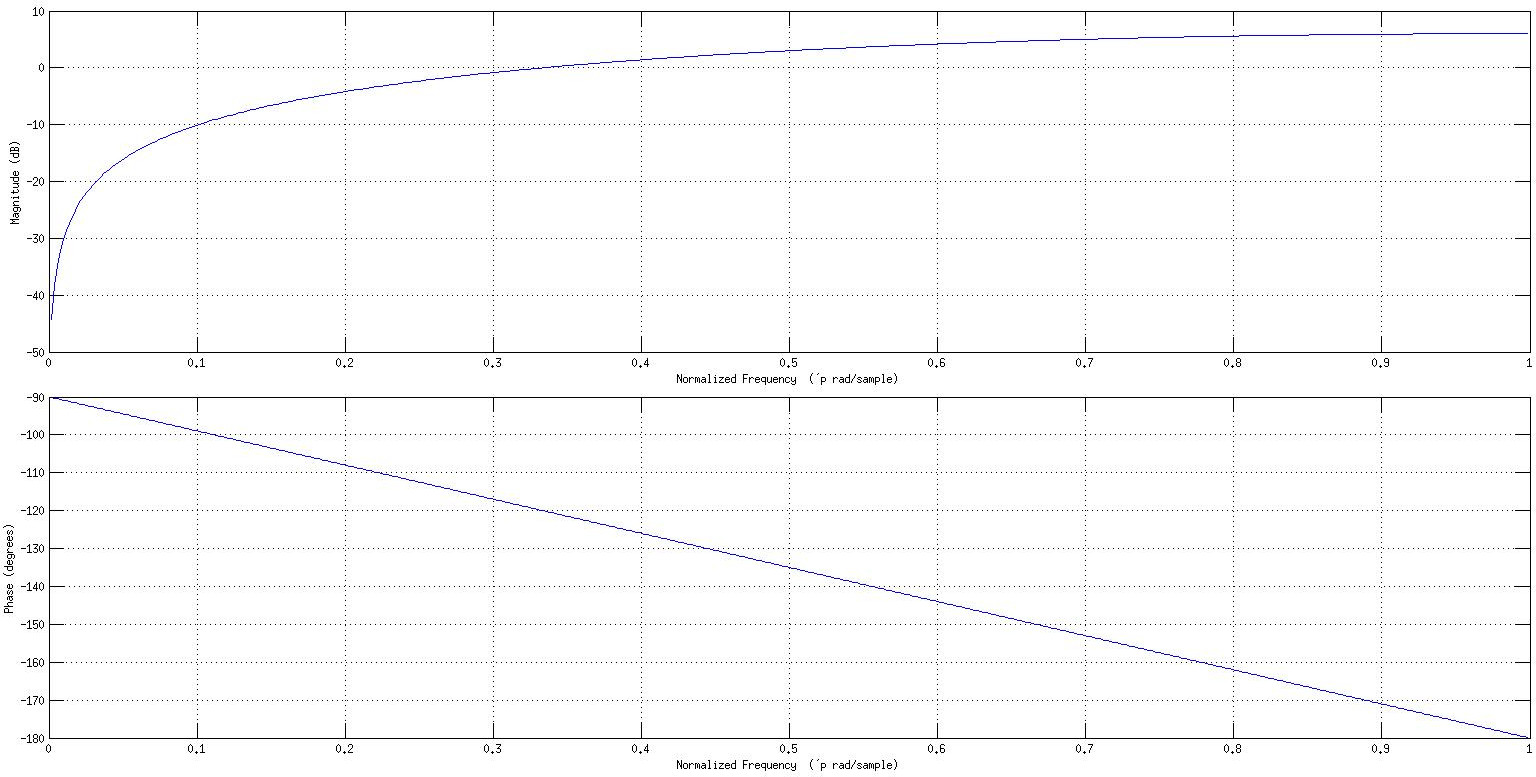
\includegraphics[width=0.8\textwidth]{pic/a3_2_5.jpg}\\
    \caption{差分的频率响应\label{a325}}
\end{figure}
代码如下:{a3\_2\_5.m}
\lstinputlisting[language=matlab]{a3_2_5.m}
\subsection{
DC 预测误差的取值和 Category 值有何关系?如何利用预测误差计算出其 Category?
}

否则$Category=ceil(log2(abs(\hat{c}_D)+1))$,包括$\hat{c}=0$的情况。

\subsection{
 你知道哪些实现 Zig-Zag 扫描的方法?请利用 MATLAB 的强大功能设
计一种最佳方法。
}
按照最原始的思路,采用循环的方式,将元素依次放入一数组中,然后利用逻辑判断决定接下来去哪个元素。但是这样速度显然很低。更为直接的思路是利用查表法,因为该图像大小为$8\times8$,直接构造一个查表矩阵是最好的,同时,通过查询\footnote{参照\url{http://blog.sina.com.cn/s/blog_54e2ed7b0100mmb7.html}},将矩阵转换到一维处理是更为简便的方式,不过其zigzag的顺序和试验要求有一定出入,简单修改即可。

代码如下(zigzag.m):
\lstinputlisting[language=matlab]{zigzag.m}
测试该函数的代码(a3\_2\_7.m)
\lstinputlisting[language=matlab]{a3_2_7.m}

\subsection{
对测试图像分块 DCT 和量化,将量化后的系数写成矩阵的形式,其中每一列为一个块的 DCT 系数 Zig-Zag 扫描后形成的列矢量,第一行为各个块的DC 系数。
}
代码如下(a3\_2\_8.m)
\lstinputlisting[language=matlab]{a3_2_8.m}
\subsection{
请实现本章介绍的 JPEG 编码(不包括写 JFIF 文件),输出为 DC 系数的
码流、 AC 系数的码流、图像高度和图像宽度,将这四个变量写入 jpegcodes.mat
文件。
}
这里二进制转换时将字符串减去48(0的ascii码),从而讲dec2bin的字符串转化成了数组。

代码如下(a3\_2\_9.m):
\lstinputlisting[language=matlab]{a3_2_9.m}
\subsection{
 计算压缩比(输入文件长度/输出码流长度),注意转换为相同进制。
}
压缩比为\[\frac{8*m*n}{length(DCstream)+length(ACstream)}\]
\[=\frac{8\times 120 \times 168}{2054+23072}=6.4188\]

\subsection{
请实现本章介绍的 JPEG 解码,输入是你生成的 jpegcodes.mat 文件。
分别用客观 (PSNR)和主观方式评价编解码效果如何。
}
生成的图像如图\ref{a3210},感觉已经很像原图了。计算得到PSNR=34.89,根据检查,haffman编码解无损(R和source一致)。
\begin{figure}
    \centering
    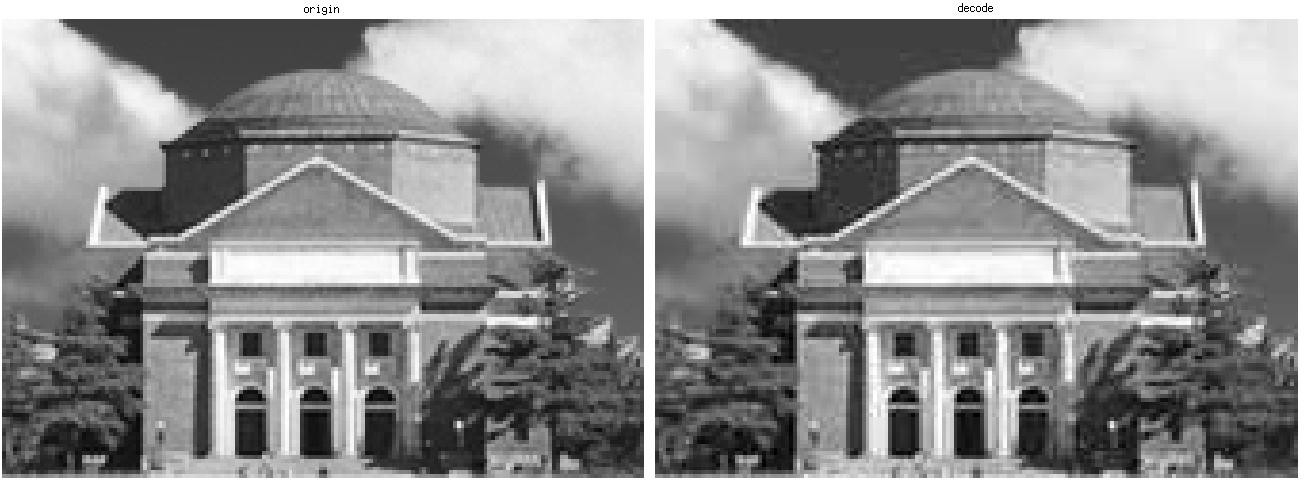
\includegraphics[width=0.8\textwidth]{pic/a3_2_10.jpg}\\
    \caption{原图与编码解码后的图像\label{a3210}}
\end{figure}

代码如下(a3\_2\_10.m):
\lstinputlisting[language=matlab]{a3_2_10.m}

\subsection{
将量化步长减小为原来的一半,重故编解码。同标准量化步长的情况比
较压缩比和图像质量。
}
使QTAB=QTAB./2即可。肉眼难以看到变化,压缩比为4.4081,PSNR为37.32。即图片效果更好了,但压缩比也小了。

\subsection{
 看电视时偶尔能看到美丽的雪花图像(见 snow.mat),请对其编解码。
和测试图像的压缩比和图像质量进行比较,并解释比较结果。
}
如图\ref{a3212},把hall\_gray换成snow即可,得到压缩比为3.6407,PSNR=29.5614。两者看起来很像,但编码解码后的图看起来颗粒要大一些,PSNR也小。
这是因为编码过程中滤去了高频分量,而雪花图像中有很强的高频分量。
\begin{figure}
    \centering
    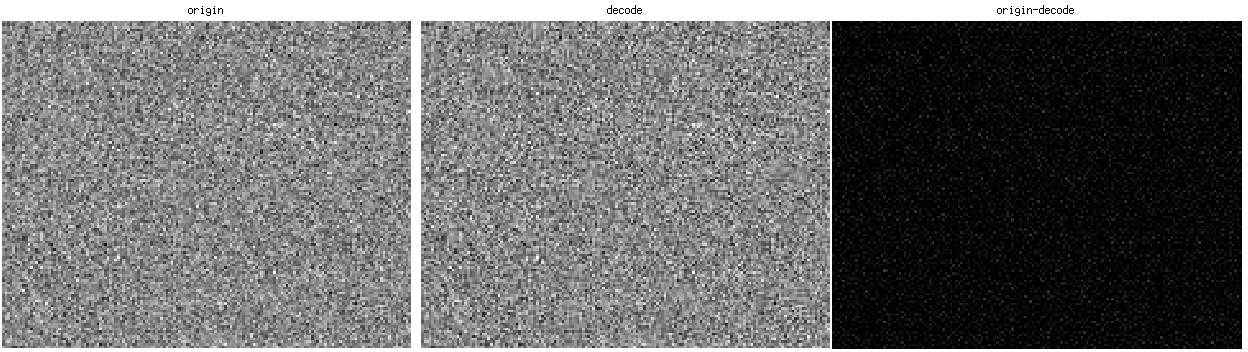
\includegraphics[width=0.8\textwidth]{pic/a3_2_12.jpg}\\
    \caption{雪花原图、编码后的图像和两者的差\label{a3212}}
\end{figure}

\section{信息隐藏}
\subsection{实现本章介绍的空域隐藏方法和提取方法。验证其抗JPEG编码能力。} 
\footnote{只处理了8bit,也就是只有英文字符,虽然增加每个字符的bit数可以加密更多的字符,但这里涉及字符编码的很多知识,在此不再进行讨论}

原始信息为传统的“A quick brown fox jump over the lazy dog。"通过图\ref{a331}可以看出隐藏很好,同时也能很好的解密信息。但是jpeg编码解码后再解密就变成了乱码\footnote{乱码形式也和字符编码有关,linux下和win下的乱码不一样,这里就不附了}。

\begin{figure}
    \centering
    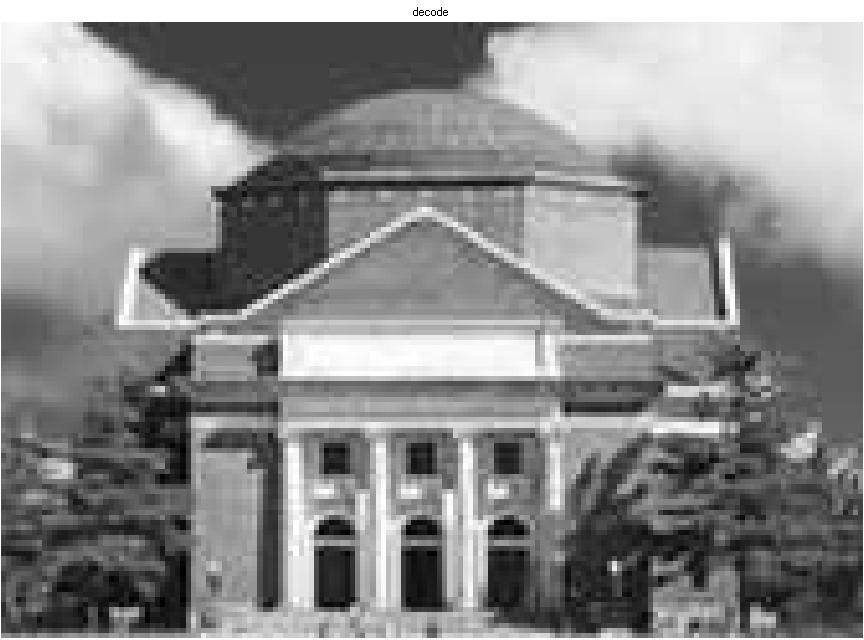
\includegraphics[width=0.3\textwidth]{pic/a3_3_1.jpg}\\
    \caption{空域隐藏\label{a331}}
\end{figure}

代码如下(a3\_3\_1.m)
\lstinputlisting[language=matlab]{a3_3_1.m}
\subsection{
依次实现本章介绍的三种变换域信息隐藏方法和提取方法,分析嵌密方法
的隐蔽性以及嵌密后 JPEG 图像的质量变化和压缩比变化。}
\footnote{把JPEG编码解码的四个过程——量化和dct(quan.m)、haffman编码(haff.m),反haffman(dehaff.m),反量化与idct(dequan.m)封装为四个函数,以方便调用}
\subsubsection{
同空域方法,用信息位逐一替换掉每个量化后的 DCT 系数的最低位,再行
熵编码。
}
信息可以很好的还原。隐藏的图像如图\ref{a332a},得到PSNR=34.6,压缩率6.29。虽然PSNR
很高,但可以明显看出左上方的噪点,这是改变前面的一部分DCT系数导致的。
\begin{figure}
    \centering
    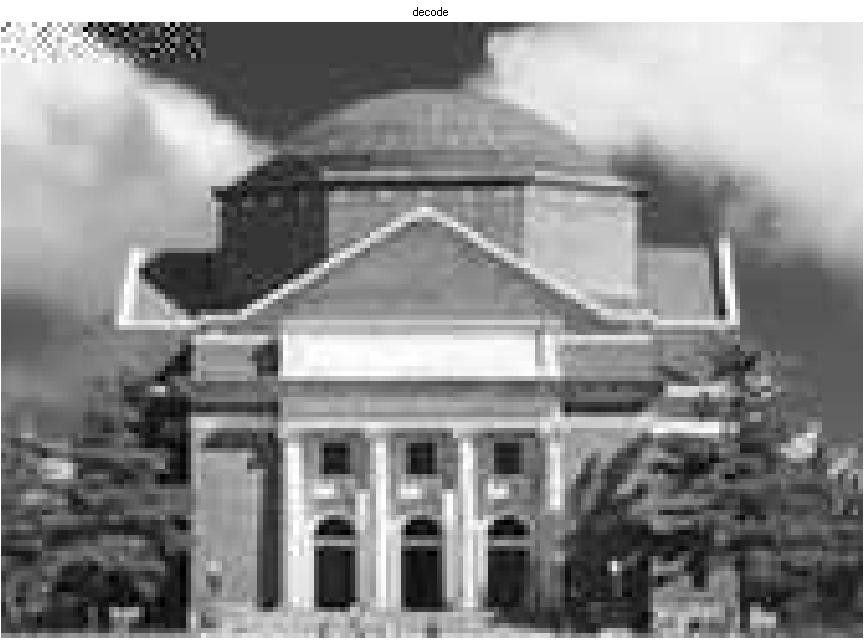
\includegraphics[width=0.5\textwidth]{pic/a3_3_2a.jpg}\\
    \caption{类似空域的DCT加密\label{a332a}}
\end{figure}
代码如下(a3\_3\_2a.m)
\lstinputlisting[language=matlab]{a3_3_2a.m}
\subsubsection{
同方法 1,用信息位逐一替换掉若干量化后的 DCT 系数的最低位,再行熵
编码。注意不是每个 DCT 系数都嵌入了信息。
}
考虑到人眼对于高频分量不敏感,将信息加载在最后两行(zigzag后的)。产生的图片如图\ref{a332b},可以看见明显的高频斑点。这是因为量化过程实际上减小了高频分量,这里在高频上增加信息在信息为1的部分相当增强了右下角的高频(第64个)信号,因此产生了类似棋盘的斑点。虽然能够恢复信息,但是加密效果并不好,图片上太明显了。

容易想到的是,合理选择被替换位可以一定程度上解决这一问题,但是下一问的方法更为合理,这里不再进行调整。
PSNR=32.24,压缩比5.49.
\begin{figure}
    \centering
    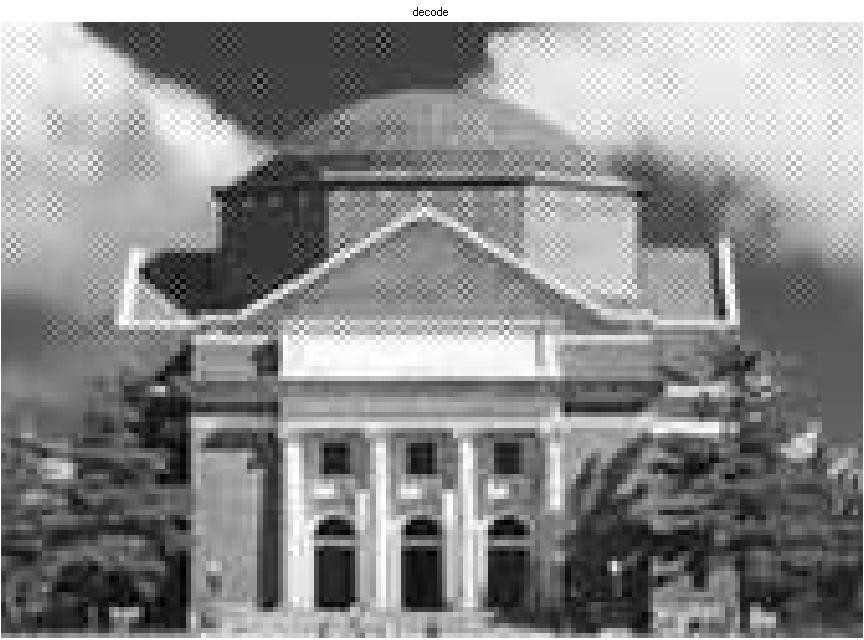
\includegraphics[width=0.5\textwidth]{pic/a3_3_2b.jpg}\\
    \caption{特定位DCT加密\label{a332b}}
\end{figure}
代码如下(a3\_3\_2a.m)
\lstinputlisting[language=matlab]{a3_3_2b.m}
\subsubsection{
先将待隐藏信息用 1, −1 的序列表示,再逐一将信息位追加在每个块 Zig-
Zag 顺序的最后一个非零 DCT 系数之后;如果原本该图像块的最后一个系数就
不为零,那就用信像息位替换该系数;
}
这一问因为是需要对zigzag的后的值逐个处理,所以将加密和解密过程分别放入haffman编码与解码的循环中。

因为整个图被分为315块,所以这种方法只能存储315bits的信息,之前的信息有些太长了,这里把信息换为经典的‘You jump I jump’。
加密后的图片如\ref{a332b},肉眼与原图不存在差异,PSNR=34.30。

\begin{figure}
    \centering
    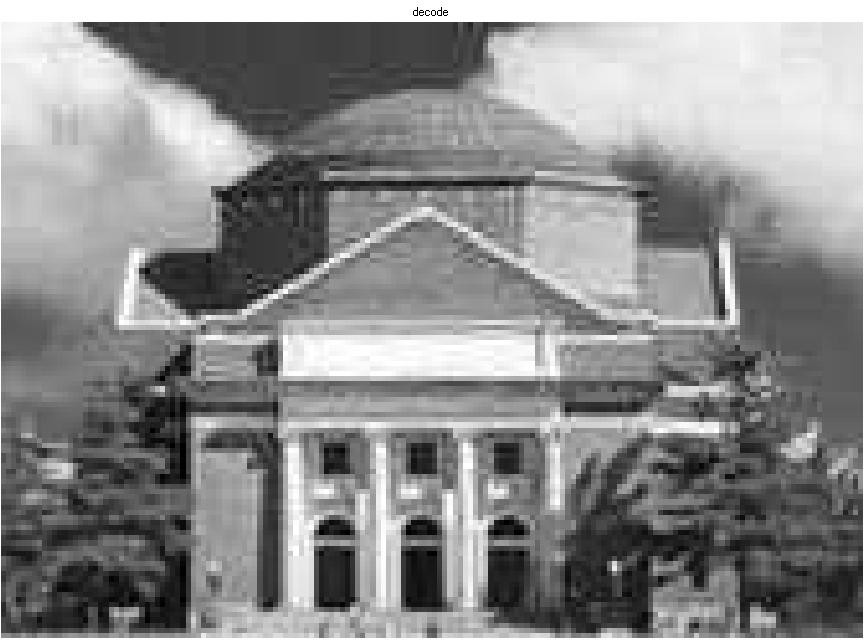
\includegraphics[width=0.5\textwidth]{pic/a3_3_2c.jpg}\\
    \caption{最后一个DCT非零系数后加密\label{a332c}}
\end{figure}
代码如下(a3\_3\_2a.m)
\lstinputlisting[language=matlab]{a3_3_2c.m}
\section{
人脸检测}
\subsection{所给资料 Faces 目录下包含从网图中截取的 28 张人脸,试以其作为样本
训练人脸标准 v}
开始时的思路是逐一遍历所有的颜色(c3),然后统计落在该颜色附近(0.5步长内)的图像点数,从而得到概率密度。但是因为颜色的数量太多,对于L,这是一个指数型的算法,实在太慢。即使我使用parpool这一并行工具箱4线程运算\footnote{这里参考了\url{http://blog.csdn.net/dang\_wang/article/details/35553953}},跑完L=5的情况还是需要5到6分钟\footnote{core i7
4800mq,仍然很慢}。在这种情况下,我甚至想到用GPU库(CUDA)去进行优化。这部分代码可以参看注释部分。

在与同学讨论这一问题时,受到同学提醒\footnote{王璞瑞同学},我发现,可以换一种思路:寻找图片的每一个点所在的颜色范围,很大程度上化简了运算。这样,计算复杂度就和L关系不大了,大大提升了计算速度,L=5的运算时间缩短到了数秒。而且由于完全是矩阵运算,没有循环,这里也不再需要使用并行算法,也很大程度上减小了程序的复杂度。这里在网上查找了histc函数的用法,以对处理过的像素点进行统计。

L=3,4,5所得值分别存储在face\_3.mat,face\_4.mat,face\_5.mat 中。
\subsubsection{样本人脸大小不一,是否需要首先将图像调整为相同大小?}
并不需要,因为这里求的是比例,和点数无关。
\subsubsection{假设 L 分别取 3, 4, 5,所得三个 v 之间有何关系?}    
其中每个的大小都是前一个的8($2^3$倍),这一点从所得到的mat文件大小也可以看出来,而相同区间的概率密度和应该是一致的。

代码如下(a3\_4\_1.m)
\lstinputlisting[language=matlab]{a3_4_1.m}

anay\_face.m代码如下
\lstinputlisting[language=matlab]{anay_face.m}
\subsection{设计一种从任意大小的图片中检测任意多张人脸的算法并编程实现(输出
图像在判定为人脸的位置加上红色的方框)。随意选取一张多人照片(比如支部
活动或者足球比赛),对程序进行测试。尝试 L 分别取不同的值,评价检测结果
有何区别。}
主要的问题是分割。这里的思路是,先在图中找到和之前所得V中出现频率最高的数种颜色相近的点,然后从这些点向四周拓展,符合条件就把index矩阵中对应的元素变为1,不符合就把这个点去掉,更换扩展范围多次重复即可。
得到图\ref{mid}。最后对index在x和y方向上分别差分即可得到边框。

这里得到的并不是一个长方形方框,而是把人脸围起来的一个不规则边框。虽然利用find函数的线性性\footnote{这部分代码见注释,看了find的help,对此没有很好的解释,但find在这里起到了这一作用}可以将其转换为标准的长方型如图\ref{a342rec},但是这样降低了准确度。
\begin{figure}
    \centering
    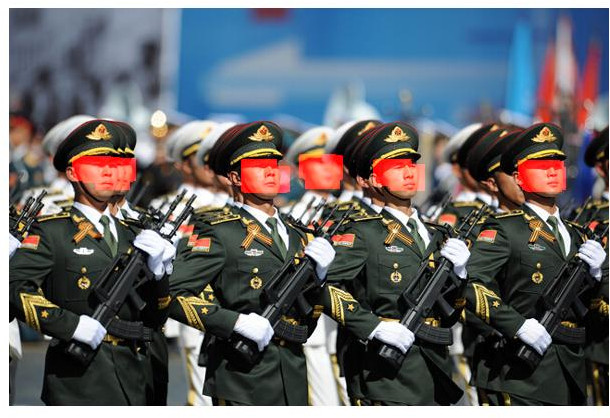
\includegraphics[width=0.5\textwidth]{pic/mid.jpg}\\
    \caption{识别中间过程\label{mid}}
\end{figure}
\begin{figure}
    \centering
    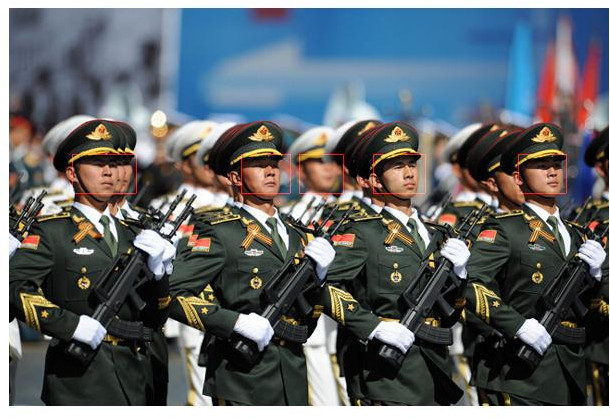
\includegraphics[width=0.5\textwidth]{pic/ex2_renc.jpg}\\
    \caption{长方形边框\label{a342rec}}
\end{figure}

还有一个问题是开始寻找点时会有很多孤立的点,它们不可能是人脸,虽然后来的变换可以消除其影响,但是太影响运算速度。这里通过在网络上查询,采用bwareaopen函数滤掉即可。

通过测试,L=4时最好的d取值为0.425,得到的图像为图\ref{a342a};L=5时最好的d取值为0.65,得到的图像为图\ref{a342b}。L3的效果较差,无法避开第三个人的脖子的同时识别后一排的人的脸,可见pic/ex2\_3.jpg文件,故没有精细调参。

可以看出,L=5时所得的框要比L=4精细很多(能分辨更小的色差),能够更好的包围住人物的脸\footnote{中间两人脸右侧多出来的框是因为后面的背景是队列的其他人,色差太小}。L=4要比L=5快大概0.3s(两者都在1s以内)。所以认为L=5的效果更好。

同时选用另一张照片进行测试,L=5,d=0.65,的到图像如图\ref{a342c},效果也不错。
\begin{figure}
    \centering
    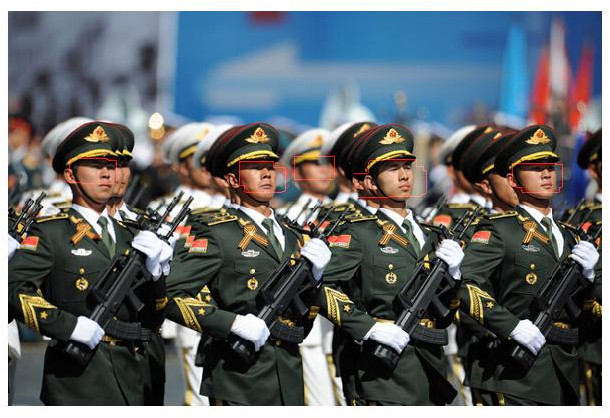
\includegraphics[width=0.5\textwidth]{pic/ex2_4_0.425.jpg}\\
    \caption{L=4,d=0.425\label{a342a}}
\end{figure}

\begin{figure}
    \centering
    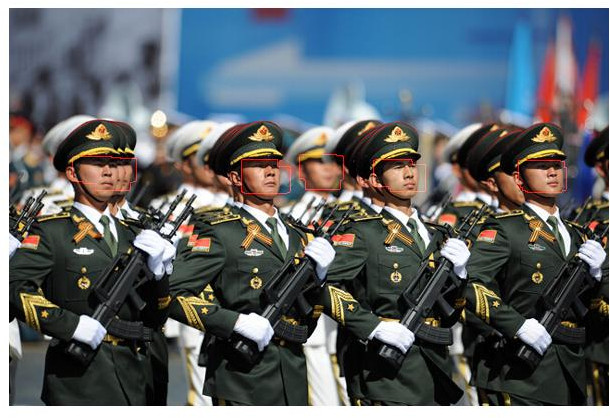
\includegraphics[width=0.5\textwidth]{pic/ex2_5_0.65.jpg}\\
    \caption{L=5,d=0.65\label{a342b}}
\end{figure}

\begin{figure}
    \centering
    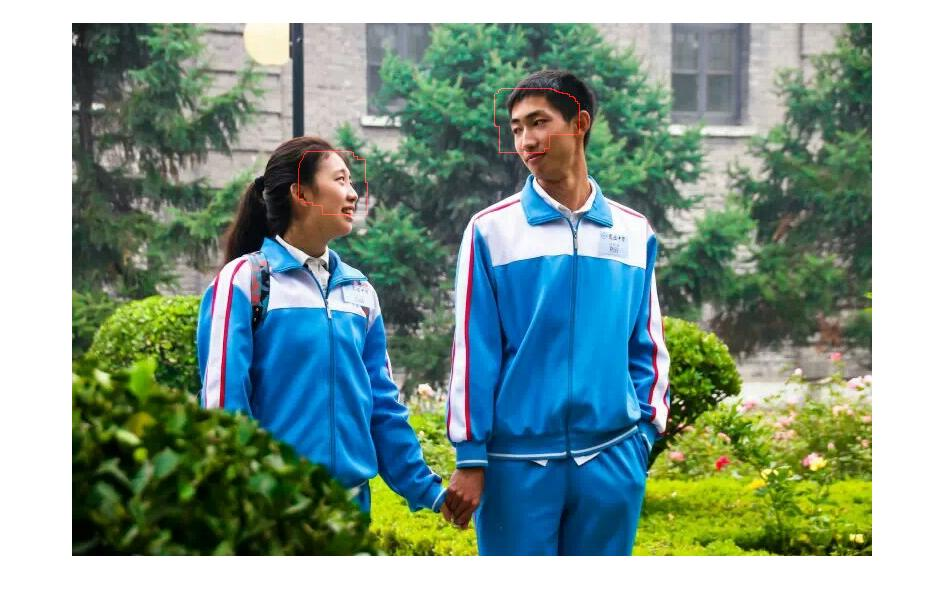
\includegraphics[width=0.5\textwidth]{pic/ex1.jpg}\\
    \caption{L=5,d=0.65\label{a342c}}
\end{figure}

代码入下(a3\_4\_2.m)
\lstinputlisting[language=matlab]{a3_4_2.m}

\subsection{对上述图像分别进行如下处理后再试试你的算法检测结果如何?并分析所得结果}
\subsubsection{顺时针旋转 90° (imrotate);}

所得图像为\ref{a343a},可以看出,红框跟着图片一起转了90°,因为本算法为检验颜色,和旋转角度无关。
旋转代码见a3\_4\_2.m第5行。
\begin{figure}
    \centering
    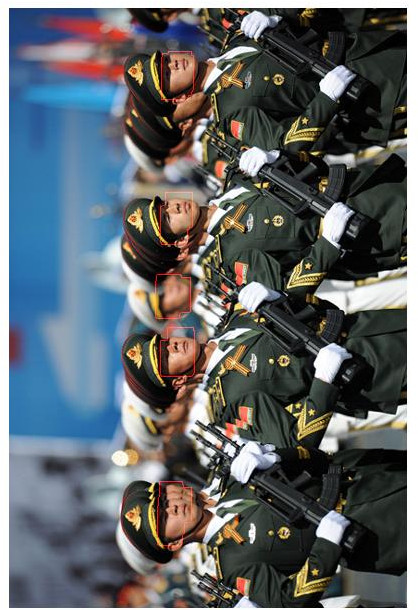
\includegraphics[width=0.4\textwidth]{pic/ex2_rotate.jpg}\\
    \caption{旋转90°\label{a343a}}
\end{figure}
\subsubsection{保持高度不变,长度拉伸为两倍}
第一次我得到的图像为\ref{a343bwrong},第二个人的脸无法被识别,debug后发现,因为我把图片转换成了double型,resize时其中出现了负数,由此导致了bug。在resize后再转换图片类型就可以解决这一bug.

修正bug后,得到图像\ref{a343bcorrect},中间两人的脖子也被标了出来,这是因为图片被拉伸后脖子相对面积变大导致的。

所用代码为a3\_4\_2.m 的9至11行。
\begin{figure}
    \centering
    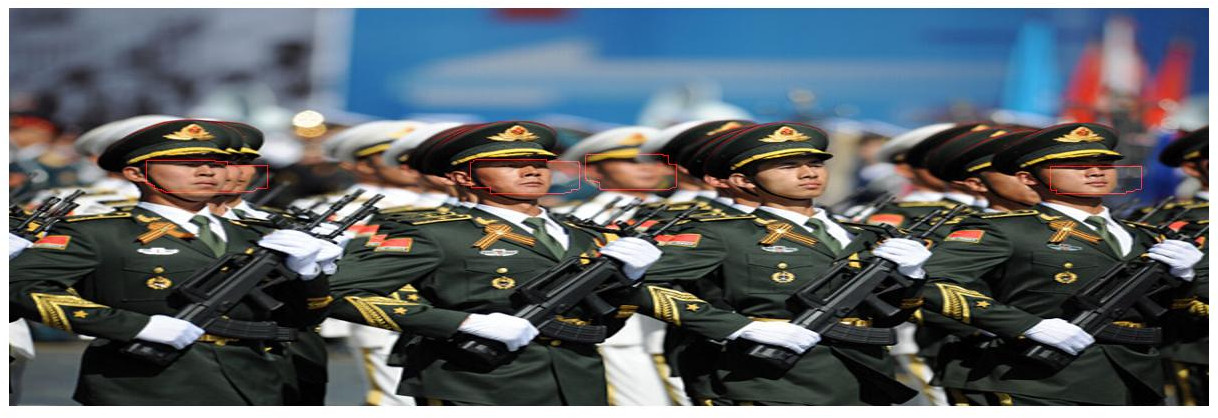
\includegraphics[width=0.8\textwidth]{pic/ex2_resize.jpg}\\
    \caption{错误的拉伸处理\label{a343bwrong}}
\end{figure}
\begin{figure}
    \centering
    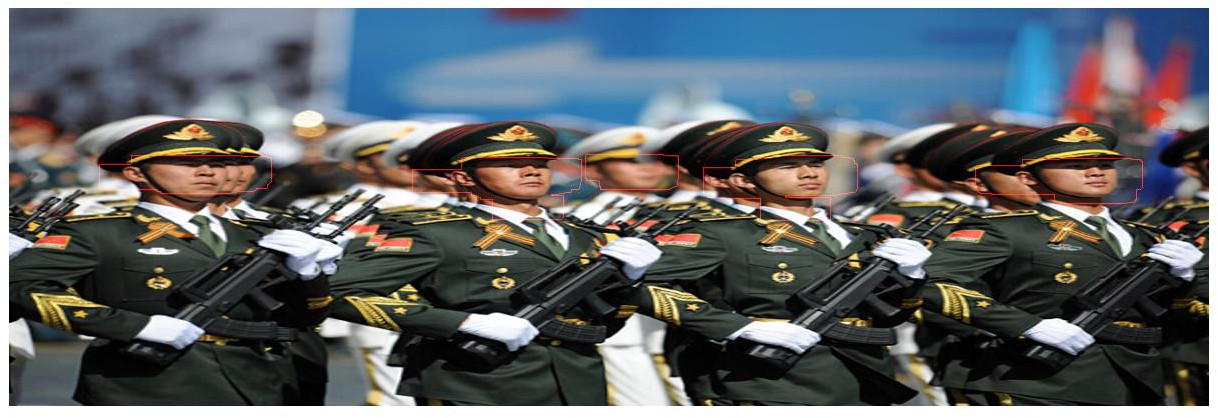
\includegraphics[width=0.8\textwidth]{pic/ex2_resize_correct.jpg}\\
    \caption{正确的拉伸处理\label{a343bcorrect}}
\end{figure}
\subsection{适当改变颜色(imadjust)}
得到图\ref{a343c},可以看到什么都没有被识别,这是因为本算法是基于颜色的,修改颜色后自然不能识别
\begin{figure}
    \centering
    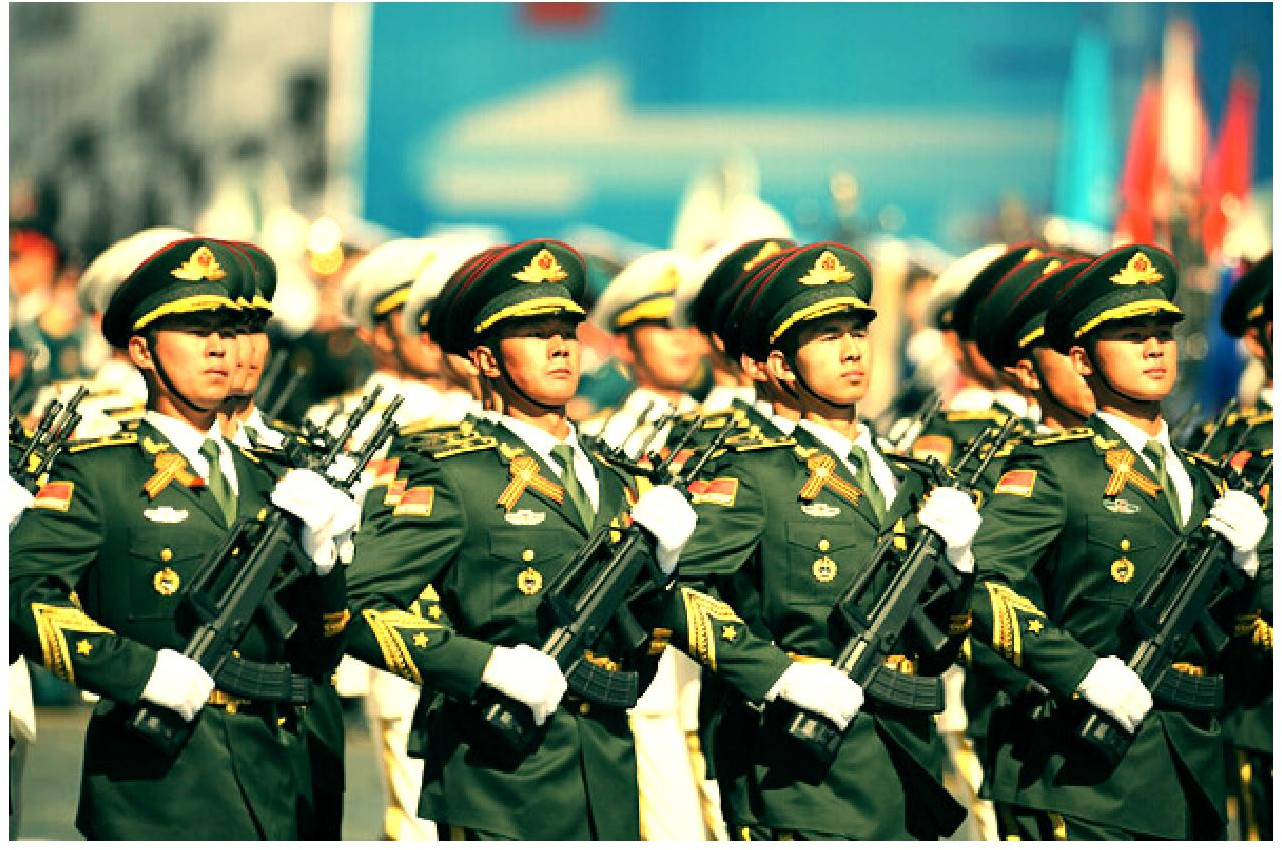
\includegraphics[width=0.5\textwidth]{pic/ex2_ad.jpg}\\
    \caption{改变颜色\label{a343c}}
\end{figure}
\subsection{如果可以重新选择人脸样本训练标准,你觉得应该如何选取}
我觉得首先应该选择单一人种的照片,胡子不能浓密,不应有眼镜、墨镜等装饰,光照应该自然(避免阴阳脸),最好分人种,分光照情况选择判定标准。
\section{总结}
本实验非常有趣,结合广泛使用的JPEG和人脸识别技术使得我更加熟悉MATLAB的矩阵运算、图像工具;也让我对图像处理的方法有了一定的认识;还让我明白图像处理多为并行处理,这也是GPU出现的原因;更难能可贵的是人脸识别部分让我理解了算法对性能的极大影响。

人脸识别的发散性题目非常有意思,在其中有过很多思路,也有很多问题和困难,最后的解决方案往往很有创意,令人兴奋。

不过在写的时候,感到自己的matlab能力还是不太扎实,一些地方还需要去网上查询,不过,多进行一些类似本实验的训练,我相信自己的能力能够得到更大的提升。

\end{document}
